\documentclass{beamer}
\usetheme{Boadilla}
\usepackage{amssymb}
\usepackage{mathtools}
\usepackage{amsmath, bm}
\usepackage{graphicx}
\usepackage[style=ieee]{biblatex}
\addbibresource{mybib.bib}


\usepackage{todonotes}
\presetkeys{todonotes}{inline}{}
\graphicspath{{./graphics/}}

\usepackage{algorithm,algorithmic}

\DeclarePairedDelimiter\norm{\lVert}{\rVert}


\setlength {\marginparwidth }{2cm}

\def\rnum{\mathbb{R}}

\title{Convex Optimisation}
\author{Alessio Zakaria}
\date{}
\begin{document}
\begin{frame}
    \titlepage
\end{frame}

\begin{frame}
    \frametitle{Structure}
    \begin{itemize}
        \item Convexity and Convex Optimisation
        \item Duality
        \item Solving Convex Optimisation Problems
            \begin{itemize}
                \item Newton's Method for Equality Constraints
                \item Barrier Method for Inequality Constraints
            \end{itemize}
    \end{itemize}
\end{frame}

\begin{frame}
    \frametitle{Convex Optimisation?}
    \begin{itemize}
    \item What is it?
        \begin{itemize}
        \item Finding the maxima / minima of convex functions over convex sets
        with respect to convex or affine constraints
        \end{itemize}
    \item Why do we care?
        \begin{itemize}
            \item Convex functions display theoretical properties that are
                suited to optimisation
            \item Solving convex optimisation problems allows you to place a lower bound
                on non-convex optimisation problems
            \item Many real world optimisation problems are convex
        \end{itemize}
    \end{itemize}
\end{frame}
\begin{frame}
    \frametitle{Convexity}
    A set $C \subseteq \mathbb{R}$ is convex if $\forall \,  x,  y \in C, \,
    \forall \, \theta \in [0, \, 1]$
    \begin{align*}
        \theta x + (1-\theta)y \in C
    \end{align*}
    i.e. all points on the line segment between $x$ and $y$ lie in C.
    \begin{figure}[t]
        \centering
        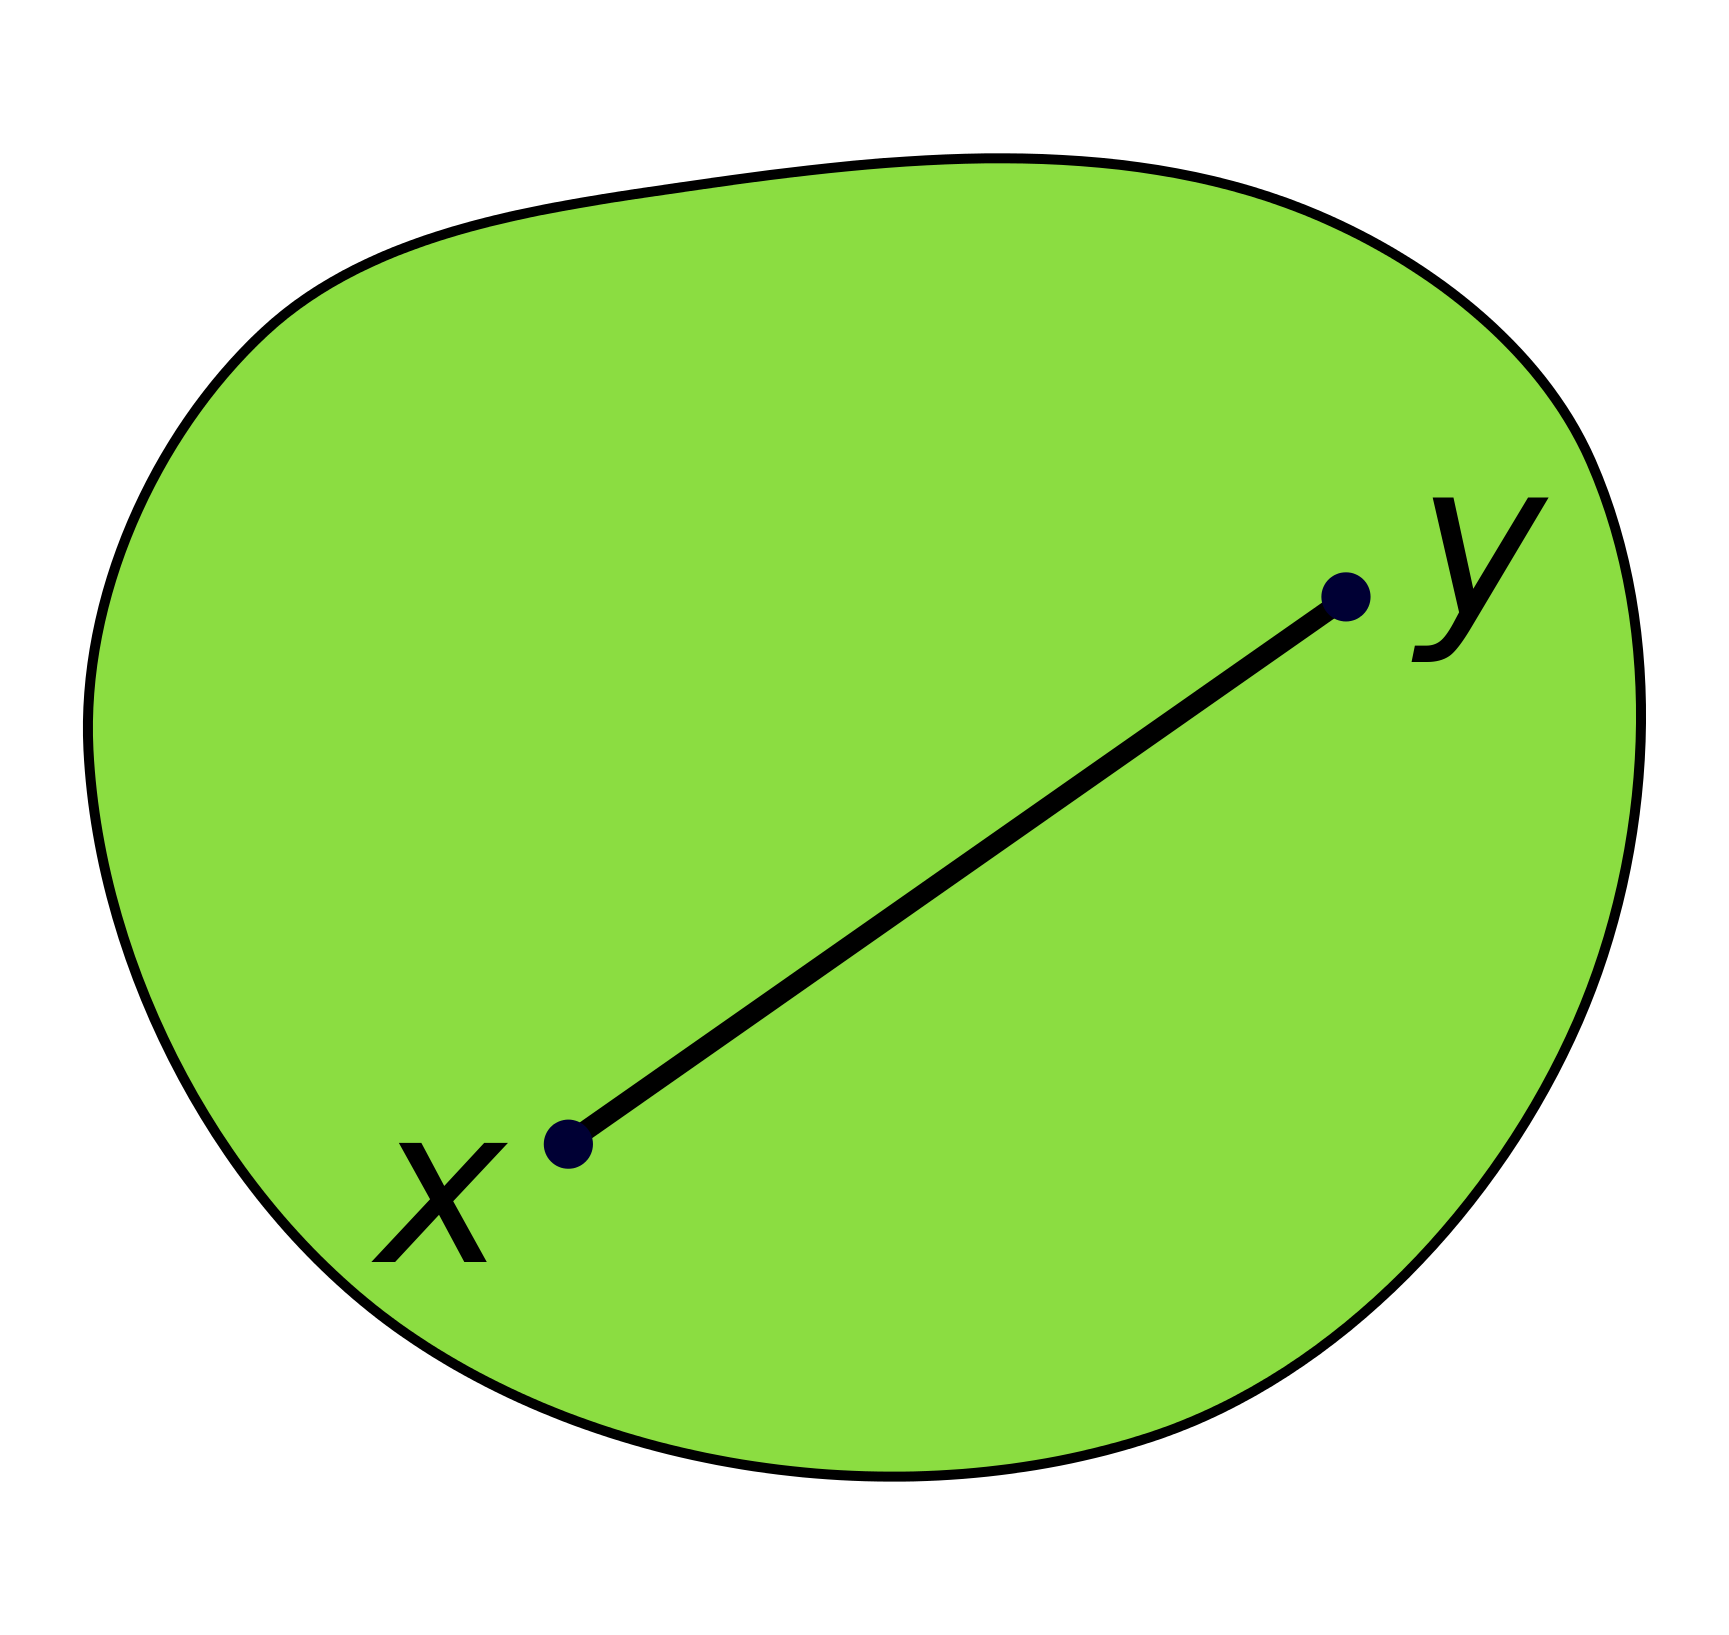
\includegraphics[scale=0.05]{polygon}
        \caption{Points in a convex set}
        \label{fig:h}
    \end{figure}
\end{frame}

\begin{frame}
    \frametitle{Convexity}
    A function $f : C \subseteq \rnum^{n} \rightarrow \rnum$ is convex iff $C$
    is a convex set and $\forall x_{1}, x_{2} \in C, \forall t \in [0,1]$
    (strict if strict equality):
    \begin{align*}
        f(t x_{1} + (1-t)x_{2}) \leq t f(x_{1}) + (1-t)f(x_{2})
    \end{align*}
    \begin{figure}[t]
        \centering
        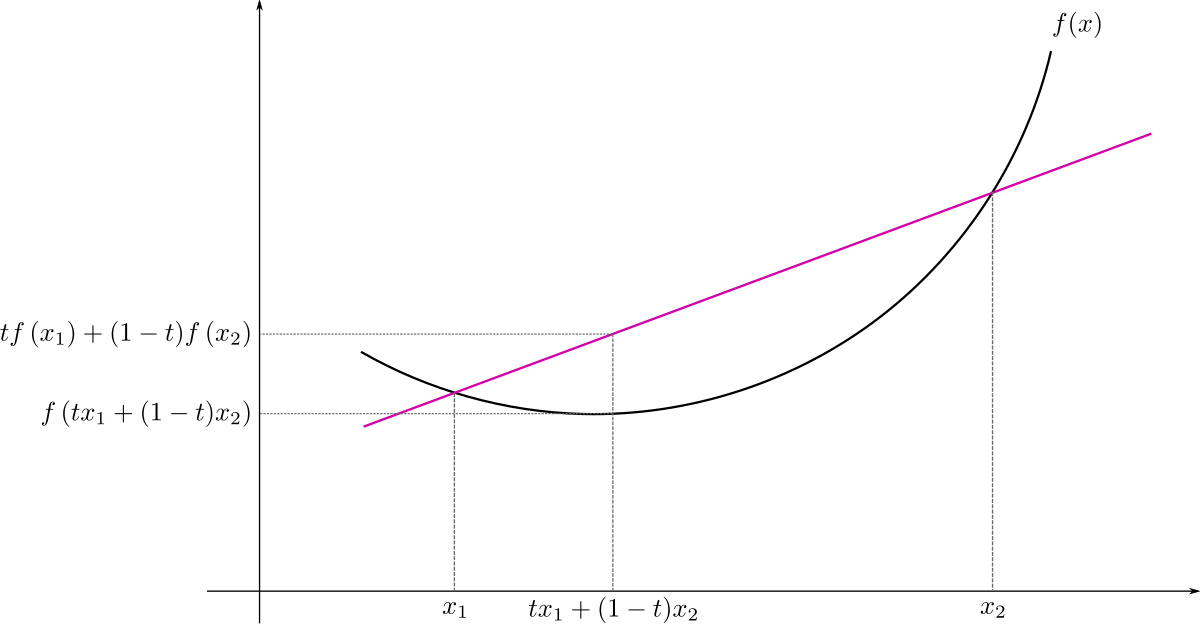
\includegraphics[scale=0.225]{function}
        \caption{A convex function}
        \label{fig:function}
    \end{figure}
\end{frame}

\begin{frame}
    \frametitle{Minima and Maxima}
    $f: S \subseteq \rnum^{n} \rightarrow \rnum$ has a global minimum (maximum
    resp.) $x^{\star}$ if:
    \begin{align*}
        \forall \, x \in S, \, \, f(x^{\star}) \leq f(x), \hspace{2mm}  (f(x^{\star}) \geq f(x))
    \end{align*}
    \\~\\
    $f$ has a local minimum (maximum resp.) around $x^{\star}$ if $\exists \, R \in
     \rnum$ \text{ such that }
    \begin{align*}
        \forall x \, \in B(x^{\star}, R), \, \, f(x^{\star}) \leq f(x),
        \hspace{2mm} (f(x^{\star}) \geq f(x))
    \end{align*}
    \\~\\
    If these inequalities are strict then $x^{\star}$ is known as a strict
    minimum (maximum)
\end{frame}

\begin{frame}
    \frametitle{Convex Optimisation Problem}
    A convex optimisation problem is a minimisation problem in the following
    form:
    {\footnotesize
    \begin{align*}
        \text{Find the }\underset{x}{\text{min}}\; &f_{0}(x) \\
        \text{  such that }&f_{1}(x) \leq 0 \\
        & \hspace{5mm} \vdots \\
        &f_{n}(x) \leq 0 \\
        &g_{0}(x) = 0 \\
        &\hspace{5mm} \vdots \\
        &g_{m}(x) = 0
    \end{align*}}
    \\~\\
    Where $f_0,\cdots, f_n$ are convex functions $\rnum^{p} \rightarrow \rnum$ and $g_0, \cdots, g_m$ are
    affine $\rnum^{p} \rightarrow \rnum$.
\end{frame}

\begin{frame}
    \frametitle{Feasible Set}
    The feasible set
    \begin{align*}
    C \subseteq D =
    \bigcap\limits_{i=0}^{m}\text{dom}(f_{i})\bigcap\limits_{j=0}^{n}\text{dom}(g_{j})
    \end{align*}
    is the set of all $x \in D$ such that the constraints are satisfied.
    \\~\\
    The \textit{optimal value} of problem is $\text{inf} \{f_{0}(x) \, | \, x
    \in C \}$. If there is no lower bound the optimisation problem has optimal
    value $-\infty$.
    \\~\\
    The point in the feasible set, $x \in C$, that attains the optimal value
    under the objective is called the \textit{optimal solution}.
\end{frame}

\begin{frame}
    \frametitle{Feasible Set}
    Some important properties of convexity are:
    \begin{itemize}
        \item The intersection of convex sets is convex
        \item The sublevel sets ($\{x \, | \, f(x) \leq 0 \}$) of convex
            functions are convex
        \item The preimage of affine functions is convex
    \end{itemize}
    Because of this the feasible set of of a convex optimisation problem is
    convex.
\end{frame}

\begin{frame}
    \frametitle{Convexity and Optimality}
    The above is important because of the following key fact:
    \\~\\
    Any local minimum of a convex function over a convex set is a global
    minimum
    \\~\\
    This means that any algorithm for a convex optimisation problem only has to
    find a local minimum.
    \\~\\
    This guarantees that algorithms which are only
    guaranteed to find local minima for all problems provide global minima for
    convex problems.
\end{frame}

\begin{frame}
    \frametitle{Characterisations of Convexity}
    First Order Characterisation of Convexity: $f : \rnum^{n} \rightarrow \rnum$
    differentiable is convex iff \textbf{dom}$(f)$ is convex and $\forall \, x
    \, y \in$ \textbf{dom}$(f)$:
    \begin{align*}
        f(y) \geq f(x) + \nabla f(x)^{T}(y-x)
    \end{align*}
    i.e. the tangent plane underapproximates the function at every point.
    \begin{figure}[t]
        \centering
        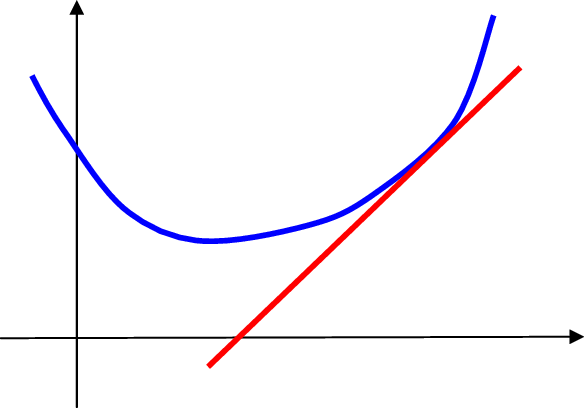
\includegraphics[scale=0.2]{tangent}
        \caption{Tangent line to a convex function}
        \label{fig:tangent}
    \end{figure}
\end{frame}

\begin{frame}
    \frametitle{Characterisations of Convexity}
    First Order Characterisation of Convexity: $f : \rnum^{n} \rightarrow \rnum$
    differentiable is convex iff \textbf{dom}$(f)$ is convex and $\forall \, x
    \, y \in$ \textbf{dom}$(f)$:
    \begin{align*}
        f(y) \geq f(x) + \nabla f(x)^{T}(y-x)
    \end{align*}
    i.e. the tangent plane underapproximates the function at every point.
    \\~\\
    Second Order Characterisation of Convexity: $f : \rnum^{n} \rightarrow
    \rnum$ twice differentiable is convex iff \textbf{dom}$(f)$ is convex and
    \begin{align*}
        \nabla^{2}f \succeq 0
    \end{align*}
    i.e. the Hessian of $f$ is positive semidefinite at all points.
\end{frame}


\begin{frame}
    \frametitle{Examples of Convex Optimization Problems}
    Various optimisation problems are convex optimization problems:
    \begin{itemize}
        \item Linear Programming
        \item Quadratic Programming with linear or convex quadratic constraints
        \item Least Squares
    \end{itemize}
\end{frame}

\begin{frame}
    \frametitle{Application: Norm Approximation}
    An optimisation problem that occurs repeatedly in statistics is norm
    approximation.
    \begin{align*}
        \underset{x}{\text{ minimise }}\norm{Ax - b}
    \end{align*}
    $A \in \rnum^{m\times n}$, $x \in \rnum^{n}$ and $b \in \rnum^{b}$.
    \\~\\
    This problem appears in many statistical estimation tasks e.g. maximum
    likelihood estimation for simple linear regression. This problem is convex
    for all norms.
\end{frame}


\begin{frame}
    \frametitle{Application: Regularisation and Optimisation}
    Regularisation is an approach to constraining the parameters of the norm
    minimisation somehow using an additive term on the objective. This appears
    in statistics when some prior information is known about the solution to the
    parameters i.e. through the choice of prior in MAP estimates:
    \begin{align*}
        \underset{x}{\text{minimise }} \norm{Ax - b}+ \gamma\norm{x}
    \end{align*}
    This can be reframed as a convex constrained optimisation problem i.e. for
    $L_{2}$ regularisation we can see this as the constrained optimisation
    problem:
    \begin{align*}
        &\underset{x}{\text{minimise }} \norm{Ax - b}
        &s.t. \norm{x}^{2} - c \leq 0
    \end{align*}
    As in Tikhonov regression
\end{frame}

\begin{frame}
    \frametitle{Duality and the Lagrangian}
    For any optimisation problem there is a related problem known as the dual
    (with the original problem known as the primal).
    \\~\\
    The solution to the dual provides some information about the solution to the
    primal.
    \\~\\
    The dual problem is always convex and therefore being able to solve
    convex optimisation problems allows us to solve the dual.
\end{frame}

\begin{frame}
    \frametitle{Duality}
    Consider some optimisation problem:
    {\footnotesize
    \begin{align*}
        \text{Find the }\underset{x}{\text{min}}\; &f_{0}(x) \\
        \text{  such that }&f_{1}(x) \leq 0 \\
        & \hspace{5mm} \vdots \\
        &f_{n}(x) \leq 0 \\
        &g_{0}(x) = 0 \\
        &\hspace{5mm} \vdots \\
        &g_{m}(x) = 0
    \end{align*}}
    Where $f_0,\cdots, f_n, g_0, \cdots, g_m:\, \rnum^{p} \rightarrow \rnum$
\end{frame}

\begin{frame}
    \frametitle{The Lagrangian}
    The Lagrangian, $L : \rnum^{p} \times \rnum^{n} \times \rnum^{m} \rightarrow
    \rnum$, of this optimisation problem is the function:
    \begin{align*}
        L(x, \lambda, \mu) = f_{0}(x) + \sum\limits_{i=1}^{n}\lambda_{i} f_{i}(x) +
        \sum\limits_{j=0}^{m}\mu_{j}g_{j}(x)
    \end{align*}
    The parameters $\lambda$ and $\mu$ are known as the Lagrangian multipliers
\end{frame}

\begin{frame}
    \frametitle{The Dual Function}
    The Dual Function $L^{\star}: \rnum^{n}\times\rnum^{m} \rightarrow \rnum$ is
    the function
    \begin{align*}
        L^{\star}(\lambda, \mu) = \underset{x \in D}{\text{min}}L(x, \lambda, \mu)
    \end{align*}
    For any feasible point of the primal $x$, for all values
    $\lambda \geq 0$, $\forall \mu$
    \begin{align*}
        L^{\star}(\lambda, \mu) \leq f_{0}(x)
    \end{align*}
    We call $(\lambda, \mu)$ dual feasible iff
    \begin{align*}
        \lambda \geq 0 \text{ and } L^{\star}(\lambda, \mu) > -\infty
    \end{align*}
\end{frame}

\begin{frame}
    \frametitle{The Dual Problem}
    Given that the values of the dual function lower bound the optimal solution
    for the primal we can formulate the question of what the greatest lower
    bound is.
    \\~\\
    This leads to the optimisation problem.
    {\footnotesize
    \begin{align*}
        \text{maximise } \, &L^{\star}(\lambda, \mu)\\
        \text{such that } &\lambda \geq 0
    \end{align*}}
    \hspace{-1mm}With optimal value $g^{\star}$ which is less than $f_{0}(x)$ for any
    $x$ in the feasible set for the primal including the optimal value i.e.
    $g^{\star} \leq p^{\star}$.
    \\~\\
    Dual feasible points are points that are (thankfully) feasible for the dual
    problem.

\end{frame}

\begin{frame}
    \frametitle{Duality}
    Regardless of whether the primal problem is convex the dual problem is
    \textit{always} convex.
    \\~\\
    This means that if convex optimisation problems can be solved efficiently
    then a lower bound can be placed on any optimisation problem that may be
    harder to solve.
    \\~\\
    This can be used in and of itself but can also be used to derive stopping
    conditions on algorithms aiming to solve the primal e.g.
    \\~\\
    For a given
    feasible point $x$ we know that the solution to the primal $p^{\star}$ lies
    between $f_{0}(x)$ and the solution to the dual $g^{\star}$. We therefore know that $x$
    is at most ($f_{0}(x) - g^{\star}$)-suboptimal.
\end{frame}

\begin{frame}
    \frametitle{Strong Duality}
    If the solution to the primal is the same as the solution to the dual
    then we say that \textit{strong duality} holds.
    \\~\\
    For convex problems if the feasible region has an interior point (known as
    Slater's condition) then strong duality holds.
    \\~\\
    If strong duality holds then the solution to the primal $x^{\star}$
    maximises the Lagrangian with respect to the solution of the dual i.e.
    $\lambda^{\star}$ and $\mu^{\star}$ i.e.
    \begin{align*}
        x^{\star} = \underset{x}{\text{min }} L(x, \lambda^{\star}, \mu^{\star})
    \end{align*}
\end{frame}

\begin{frame}
    \frametitle{Solving Convex Optimisation Problems}
    One method of solving convex optimisation problems is using interior point
    methods.
    \\~\\
    Intuition: Reformulate the problem as an equality constrained problem which
    can be solved via Newton's Method
\end{frame}

\begin{frame}
    \frametitle{Newton's Method}
    Newton's method is an iterative method for solving unconstrained minimisation problems:
    \begin{itemize}
        \item For twice differentiable functions
        \item Uses the Hessian to take into account local curvature information
    \end{itemize}
    To find a minimum of some twice differentiable $f(x)$ with gradient $\nabla
    f(x)$ and Hessian $\nabla^{2}f(x)$ take iterative
    steps.
\end{frame}

\begin{frame}
    \frametitle{Newton's Method}
    At point $x_{n}$, set $x_{n+1} = x_{n} + \lambda \Delta x$. $\Delta x$ is set
    using the second order Taylor's approximation as follows:

    \begin{align*}
        \Delta x = \underset{\Delta x \in \rnum^{d}}{\text{argmin}}\, \,f(x + \Delta
        x) = \underset{\Delta x \in \rnum^{d}}{\text{argmin}} \, \, f(x) + \nabla f(x)^{T}
        \Delta x + \frac{1}{2}\Delta x^{T}\nabla^{2}f(x)\Delta x
    \end{align*}
    \\~\\
    Taking the derivative of the final expression, equating to 0 and solving for
    $\Delta x$ we obtain:
    \begin{align*}
        \Delta x = -(\nabla^{2}f(x))^{-1}\nabla f(x)
    \end{align*}
\end{frame}


\begin{frame}
    \frametitle{Newton's Method for Equality Constrained Optimisation}
    Newton's Method can be used to find the minima of functions according to
    equality constraints i.e.
    \begin{align*}
        &\underset{x}{\text{minimise }}  f(x) \\
        &\text{such that } A x = b
    \end{align*}
    where $f : \rnum^{m} \rightarrow \rnum$ twice differentiable, $A \in \rnum^{n \times m} $
    where $\Delta x$ is calculated with the $2^{\text{nd}}$ order Taylor Approximation:
    {\footnotesize
    \begin{align*}
        \Delta x &= \underset{\Delta x \in \rnum^{d}}{\text{argmin}}\, \,f(x + \Delta
        x)  \\
        &= \, \underset{\Delta x \in \rnum^{d}}{\text{argmin}} \, \, f(x) + \nabla f(x)^{T}
        \Delta x + \frac{1}{2}\Delta x^{T}H(x)\Delta x \\ \vspace{1mm}
        &\,\,\,\,\,\, \text{             such that } A\, (x + \Delta x) = b
    \end{align*}}
    Which is a quadratic constrained minimisation problem.
\end{frame}

\begin{frame}
    \frametitle{Newton's Method for Equality Constrained Optimisation}
    If $f$ is convex (and Slater's constraint holds) then strong duality holds
    assuming that a minimum exists at some $x^{\star}$.
    \\~\\
    Forming the Lagrangian for an equality constrained problem we
    obtain:
    \begin{align*}
        L(x, v) = f(x) + A^{T}v
    \end{align*}
    Since $x^{\star}$ minimizes $L(x, v^{\star} )$ over x, it follows that
    its gradient must vanish at $x^{\star}$ , i.e.
    \begin{align*}
        0 = \nabla f(x^{\star}) -  \nabla A^{T}v^{\star} \\
        \nabla f(x^{\star}) = \nabla A^{T}v^{\star} \\
        \nabla f(x^{\star}) = A^{T} v^{\star}
    \end{align*}
\end{frame}

\begin{frame}
    \frametitle{Newton's Method for Equality Constrained Optimisation}
    We therefore have two constraints that must be satisfied for minimum
    $x^{\star}$.
    \begin{align*}
        &\nabla f(x^{\star}) = A^{T} v^{\star} \text{ and} \\
        &A x^{\star} = b
    \end{align*}
    Replacing $x^{\star}$ with $x + \Delta x$ using the $2^{\text{nd}}$ order
    Taylor approximation of the original $f$ the constraints become:
    \begin{align*}
        &\nabla^{2}f(x)\Delta x + \nabla f(x) = A^{T}v \text{ and}\\
        &A(x + \Delta x) = b
    \end{align*}
    Which, if $Ax = b$ gives rise to the KKT system:
    \begin{align*}
        \begin{bmatrix}
            \nabla^{2}f(x) & A^{T} \\
            A & 0
        \end{bmatrix}
        \begin{bmatrix}
            \Delta x \\
            v
        \end{bmatrix}
        =
        \begin{bmatrix}
            -\Delta f(x) \\
            0
        \end{bmatrix}
    \end{align*}
\end{frame}

\begin{frame}
    \frametitle{Newton's Method for Equality Constrained Optimisation}
    Newton's method has quadratic convergence for a strictly convex $f$ and
    Lipschitz continuous Hessian (faster than gradient descent)
    even for the equality constrained version, however it has high complexity and
    memory usage for each iteration as it must store the whole Hessian
    $(O(n^{2}))$ and calculate its inverse $(O(n^{3}))$.
    \\~\\
    The algorithm also requires a feasible starting point i.e. some $x$ such
    that $A x = b$. The algorithm can be adapted to support starting from an
    infeasible point.
\end{frame}

\begin{frame}
    \frametitle{Solving Inequality Constrained Optimisation}
    We now know how to deal with equality constraints in convex optimisation
    problems. Now it remains to deal with inequality constraints.
    We incorporate the inequalities into the objective using an indicator
    function:
    \begin{align*}
        \text{minimise } \, &f_{0} +
        \sum_{i=1}^{m}\mathcal{I}\_\left(f_{i}\,(x)\right )\\
        \text{such that } & Ax =b
    \end{align*}

where

\begin{align*}
    \mathcal{I}\_(u) =
    \begin{cases}
        0 &u \leq 0 \\
        \infty &u > 0
    \end{cases}
\end{align*}
\end{frame}

\begin{frame}
    \frametitle{Solving Inequality Constrained Optimisation}
    This objective is not differentiable and therefore Newton's method cannot be
    applied.
    \\~\\
    To rectify this we can use an approximation using the log barrier function.
    \begin{align*}
        \hat{\mathcal{I}}\_\, (u) = -\frac{1}{t}\, \text{log}\,(-u) \\\\
        \mathbf{dom} \,\,\,\hat{\mathcal{I}}\_ = -\rnum^{++}
    \end{align*}
    Where $t$ is a parameter that is set to adjust the accuracy of the barrier
    function
\end{frame}

\begin{frame}
    \frametitle{Log Barrier Function}
    The minimisation problem can be reformuated as the following:
    \begin{align*}
        \text{minimise } \, &t f_{0} +
        \varphi(x)\\
        \text{such that } & Ax =b
    \end{align*}
    where
    \begin{align*}
        \varphi(x) = - \sum\limits_{i=1}^{m}\text{log}(-f_{i}(x))
    \end{align*}
    where
    \begin{align*}
        \nabla \varphi(x) = \sum\limits_{i=1}^{m}\frac{1}{-f_{i}(x)}\nabla f_{i}(x)
    \end{align*}
\end{frame}

\begin{frame}
    \frametitle{Log Barrier Function}
    \begin{figure}[t]
        \centering
        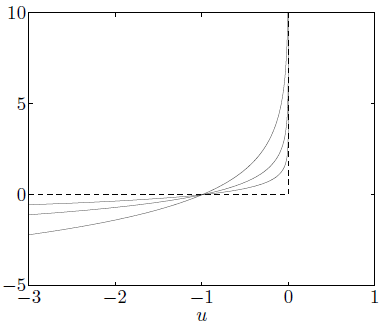
\includegraphics[scale=0.6]{barrier_function}
        \caption{log barrier function for increasing values of $t$}
        \label{fig:logbar}
    \end{figure}
    The log barrier function is twice continuously differentiable and convex
    and therefore is amenable to Newton's method.
\end{frame}


\begin{frame}
    \frametitle{Central Path}
    Before applying Newton's method however, it is useful to know what value we
    should set $t$ to. This can be found through analysing the \textit{central
    path}.
    \\~\\
    Assuming the log barrier formalisation has a unique solution for all
    $t > 0$ obtainable via Newton's method, we can define the central path,
    $x^{\star}(t)$ as the \textit{unique} solution to the minimisation problem for a given
    $t$.
    \\~\\
    From the KKT conditions a dual feasible point for every
    $x^{\star}(t)$ can be obtained which lower bounds the optimal value for
    the original problem.
\end{frame}

\begin{frame}
    \frametitle{Central Path}
    Let
    \begin{align*}
        \lambda_{i}^{\star}(t) = -\frac{1}{t f_{i}(x^{\star}(t))} \text{ and }
        v^{\star}(t) = \hat{v} / {t}
    \end{align*}
    We claim that these are dual feasible points for the dual function
    \begin{align*}
        g(\lambda(t), v(t)) &= \underset{x(t)}{\text{min }}f_{0}(x(t))
        + \sum\limits_{i=1}^{m}\lambda_{i}(t)f_{i}(x(t))
        + v(t)^{T}(Ax(t) - b) \\
    \end{align*}
    and that $x^{\star}(t)$ is the value of $x(t)$ that minimises the above for
    $\lambda_{i}^{\star}(t)$ and $v^{\star}(t)$.
\end{frame}

\begin{frame}
    \frametitle{Central Path}
    If this is true then
    {\footnotesize
        \begin{align*}
            g(\lambda^{\star}(t), v^{\star}(t)) &= f_{0}(x^{\star}(t))
            + \sum\limits_{i=1}^{m}\lambda_{i}^{\star}(t)f_{i}(x^{\star}(t))
            + v^{\star}(t)^{T}(Ax^{\star}(t) - b) \\
        \end{align*}
    }
    \vspace{-10mm}
    \begin{align*}
        \hspace{-10mm}\text{As }\hspace{5mm}  Ax^{\star}(t) = b \text{ and } \lambda_{i}^{\star}(t)f_{i}(x^{\star}(t))
        = -\frac{f_{i}(x^{\star}(t))}{t f_{i}(x^{\star}(t))}
        = -\frac{1}{t}
    \end{align*}
    \begin{align*}
        g(\lambda^{\star}(t), v^{\star}(t)) &= f_{0}(x^{\star}(t)) -
        \frac{m}{t}
    \end{align*}
    This means that for a given $x^{\star}(t)$, $f_{0}(x^{\star}(t))$ is no more than
    $\frac{m}{t}$ away from the optimal value for the original primal problem.
\end{frame}

\begin{frame}
    \frametitle{Central Path}
    We claimed that $\lambda^{\star}(t)$ and $v^{\star}(t)$ were dual feasible
    points for the dual. To show this observe the following:
    \\~\\
    Points on the central path are characterised by the KKT conditions:
    {\footnotesize
    \begin{align*}
        \exists \hat{v}\,\, s.t.  \, \, \,\, \, \, \,
        0 &= t\nabla f_{0}(x^{\star}(t)) + \nabla\phi(x^{\star}(t)) +
        A^{T}\hat{v} \\
        &= t \nabla f_{0}(x^{\star}(t)) +
        \sum\limits_{i=1}^{m}\frac{1}{-f_{i}(x^{\star}(t))}\nabla
        f_{i}(x^{\star}(t)) + A^{T}\hat{v}
    \end{align*}}
    This can be observed to be the derivative of the Lagrangian where $\lambda =
    \lambda^{\star}(t)$ and $v = v^{\star}(t)$. As this equals 0 this means that
    the dual function is bounded below for $\lambda^{\star}(t)$ and
    $v^{\star}(t)$.
\end{frame}

\begin{frame}
    \frametitle{Central Path}
    The other condition for dual feasibility is that $\lambda^{\star}(t) >
    0$.
    \\~\\
    As $f_{i}(x^{\star}) < 0$ for $x^{\star}$ then
    \begin{align*}
        -\frac{1}{f_{i}(x^{\star})} > 0
    \end{align*}
    And therefore $\lambda^{\star}(t)$ and
    $v^{\star}(t)$ are dual feasible and the suboptimality bound holds.
\end{frame}


\begin{frame}
    \frametitle{Central Path}
    \begin{figure}[t]
        \centering
        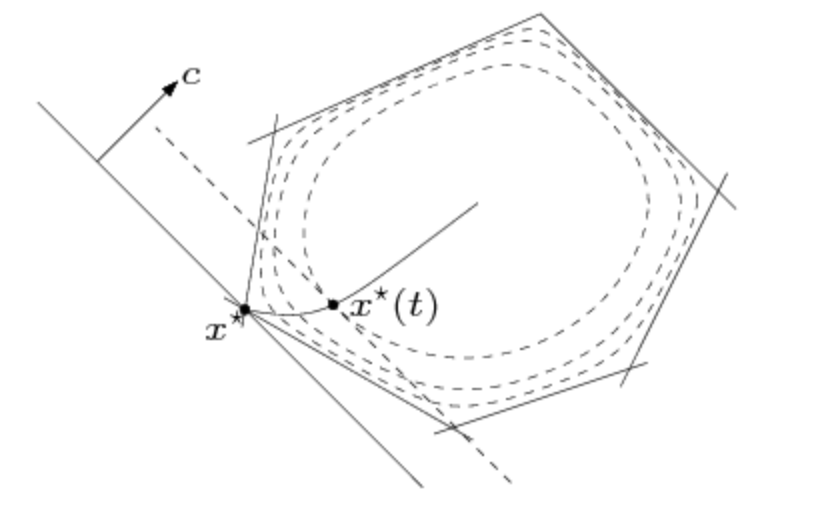
\includegraphics[scale=0.25]{central_path}
        \caption{Traversing the central path to the optimal value}
        \label{fig:central path}
    \end{figure}
    \vspace{-5mm}
    As $t \rightarrow \infty$ the central path solution will tend to
    $p^{\star}$.
\end{frame}

\begin{frame}
    \frametitle{Barrier Method}
    Given that an abitrary $x^{\star}(t)$ is $\frac{m}{t}$ suboptimal a method of
    finding the minimum of the original problem to a specific accuracy,
    $\varepsilon$ is by solving the problem:
    \begin{align*}
        \text{minimise } \, &\left(\frac{m}{\varepsilon}\right)\,f_{0} +
        \varphi(x)\\
        \text{such that } & Ax =b
    \end{align*}
    This can be solved using Newton's method however it does not have good
    practical performance due to numerical instability as when  $\varepsilon$
    is large then the value of the objectives Hessian varies rapidly near the
    boundaries of the feasible set.
\end{frame}

\begin{frame}
    \frametitle{Barrier Method}
    The barrier method avoids the problems of the previous method by solving a
    series of minimisation problems.
    \\~\\
    The barrier method computes $x^{\star}(t)$ for increasing values of
    $t$ using Newton's method until $t \geq \frac{m}{\varepsilon}$.
\end{frame}


\begin{frame}
    \frametitle{Barrier Method Algorithm}
    \begin{algorithm}[H]
        \begin{algorithmic}[1]
            \WHILE{$ m / {t}< \varepsilon$}
            \STATE $x \leftarrow \text{ minimise } tf_{0} + \phi
            \text{ such that } Ax = b \text{ starting at x}$
            \STATE $t \leftarrow \mu t$
            \ENDWHILE
        \end{algorithmic}
        \caption{Barrier Method}
        \label{alg:seq}
    \end{algorithm}
    The method of minimisation on line 2 is assumed to be Newton's Method.
    \\~\\
    The choice of $\mu$ dictates how many of the outer non-Netwon's method loop
    occur. If this is too high then Newton's method might take too long to
    converge. If $t^{(0)}$ is too small then many outer iterations may be
    needed.
    \\~\\
    The Barrier Method is quite robust to the choice of these in practice.
\end{frame}

\begin{frame}
    \frametitle{Barrier Method Analysis}
    To reach an accuracy of $\varepsilon$, assuming that Newton's Method in step
    2 returns an exact solution, requires
    \begin{align*}
        \frac{\log(m/{t^{(0)}\varepsilon)}}{\log \mu}+1
    \end{align*}
    iterations of the outer loop.
    \\~\\
    To apply the barrier method we require a strictly feasible point to begin
    the algorithm. This can be solved by a \textit{feasability} method which is
    an initial constrained convex optimisation problem for which it is easy to find a strictly
    feasible starting point such that the barrier method can applied.
\end{frame}


\begin{frame}
    \frametitle{Interior Point Methods}
    There exist more advanced interior point methods that are more efficient
    for higher accuracy than the Barrier method.
    \\~\\
    Primal-Dual methods are an active area of research for non-linear convex
    problems that are more efficient than Barrier methods.
    \\~\\
    Primal-Dual methods take one Newton step instead of the separation between
    the outer loop of the Barrier Method and updating the inner iterations of
    Newton's method.
\end{frame}

\begin{frame}
    \frametitle{Summary}
    In this talk we have:
    \begin{itemize}
        \item Learnt what a convex optimisation problem is
        \item Learnt about duality and how convex optimisation can be used to lower bound all
            optimisation problems
        \item Learnt about how Newton's Method can be adapted to solve equality
            constrained problems
        \item Learnt about how the Barrier method can be used to incorporate
            inequalities into the objective and iteratively apply Newton's
            method to solve inequality constrained problems.
    \end{itemize}
\end{frame}

\begin{frame}
    \nocite{*}
    \printbibliography
\end{frame}

\begin{frame}
    \centering
    Thanks \\
    Any Questions?
\end{frame}
% \begin{frame}
%     \frametitle{Applications: Regularised Logistic Regression}
%     There is no closed form solution for the parameters of logistic regression
%     and therefore a numerical method must be used.
%     \\~\\
%     One of the aims of regularisation is to ensure the size of the parameters
%     remain small.
%     \\~\\
%     This can be reformulated as a constrained minimisation problem.
% \end{frame}

% \begin{frame}
%     \frametitle{Applications: Regularised Logistic Regression}
%     With data $\mathbf{x}_{1},\dots,\mathbf{x}_{n} \in \rnum^{d}$ and class
%     variables $y_{1}, \dots, y_{n} \in \{0, 1\}$.
%     Model $p(y| X = x)$ as:
%     \begin{align*}
%         p(y | X = \textbf{x}) = \frac{1}{1 + e^{-y_{i} \cdot \langle \textbf{w} ,
%                 \textbf{x}'
%         \rangle}}
%     \end{align*}
%     where $\textbf{w} \in \rnum^{d+1}$ and $\textbf{x}' = [\textbf{x}, 1]^{T}$
%     \\~\\
%     Doing MLE and taking the negative log-likelihood we obtain the optimisation
%     problem
%     \begin{align*}
%        l
%     \end{align*}
% \end{frame}

% \begin{frame}
%     \frametitle{Applications: Regularised Logistic Regression}
% \end{frame}

% \begin{frame}
%     \frametitle{Strong and Weak Duality}
% \end{frame}

% \begin{frame}
%     \frametitle{Strong Duality for Convex Problems}
% \end{frame}

% \begin{frame}
%     \frametitle{Solving Convex Optimisation Problems}
% \end{frame}
\end{document}

